\subsection{Muscle Activation}
The muscle activity of the TA, GA and SOL of the contralateral leg in response to unilateral perturbations for a representative subject is shown in Fig. \ref{muscleActivityFigure}.  The mean value of muscle activity of all cycles pertaining to a surface stiffness is plotted as a function of the gait cycle percentage, where heel-strike and toe-off of the right leg are indicated on the figure as HS and TO, respectively.  The profile of walking on a rigid surface resembles that of what would be expected for normal human gait \cite{Perry_1992_Gait}, therefore our system did not alter normal gait patterns.

\begin{figure}
\centering
\begin{subfigure}{1.0\columnwidth}
	\centering
	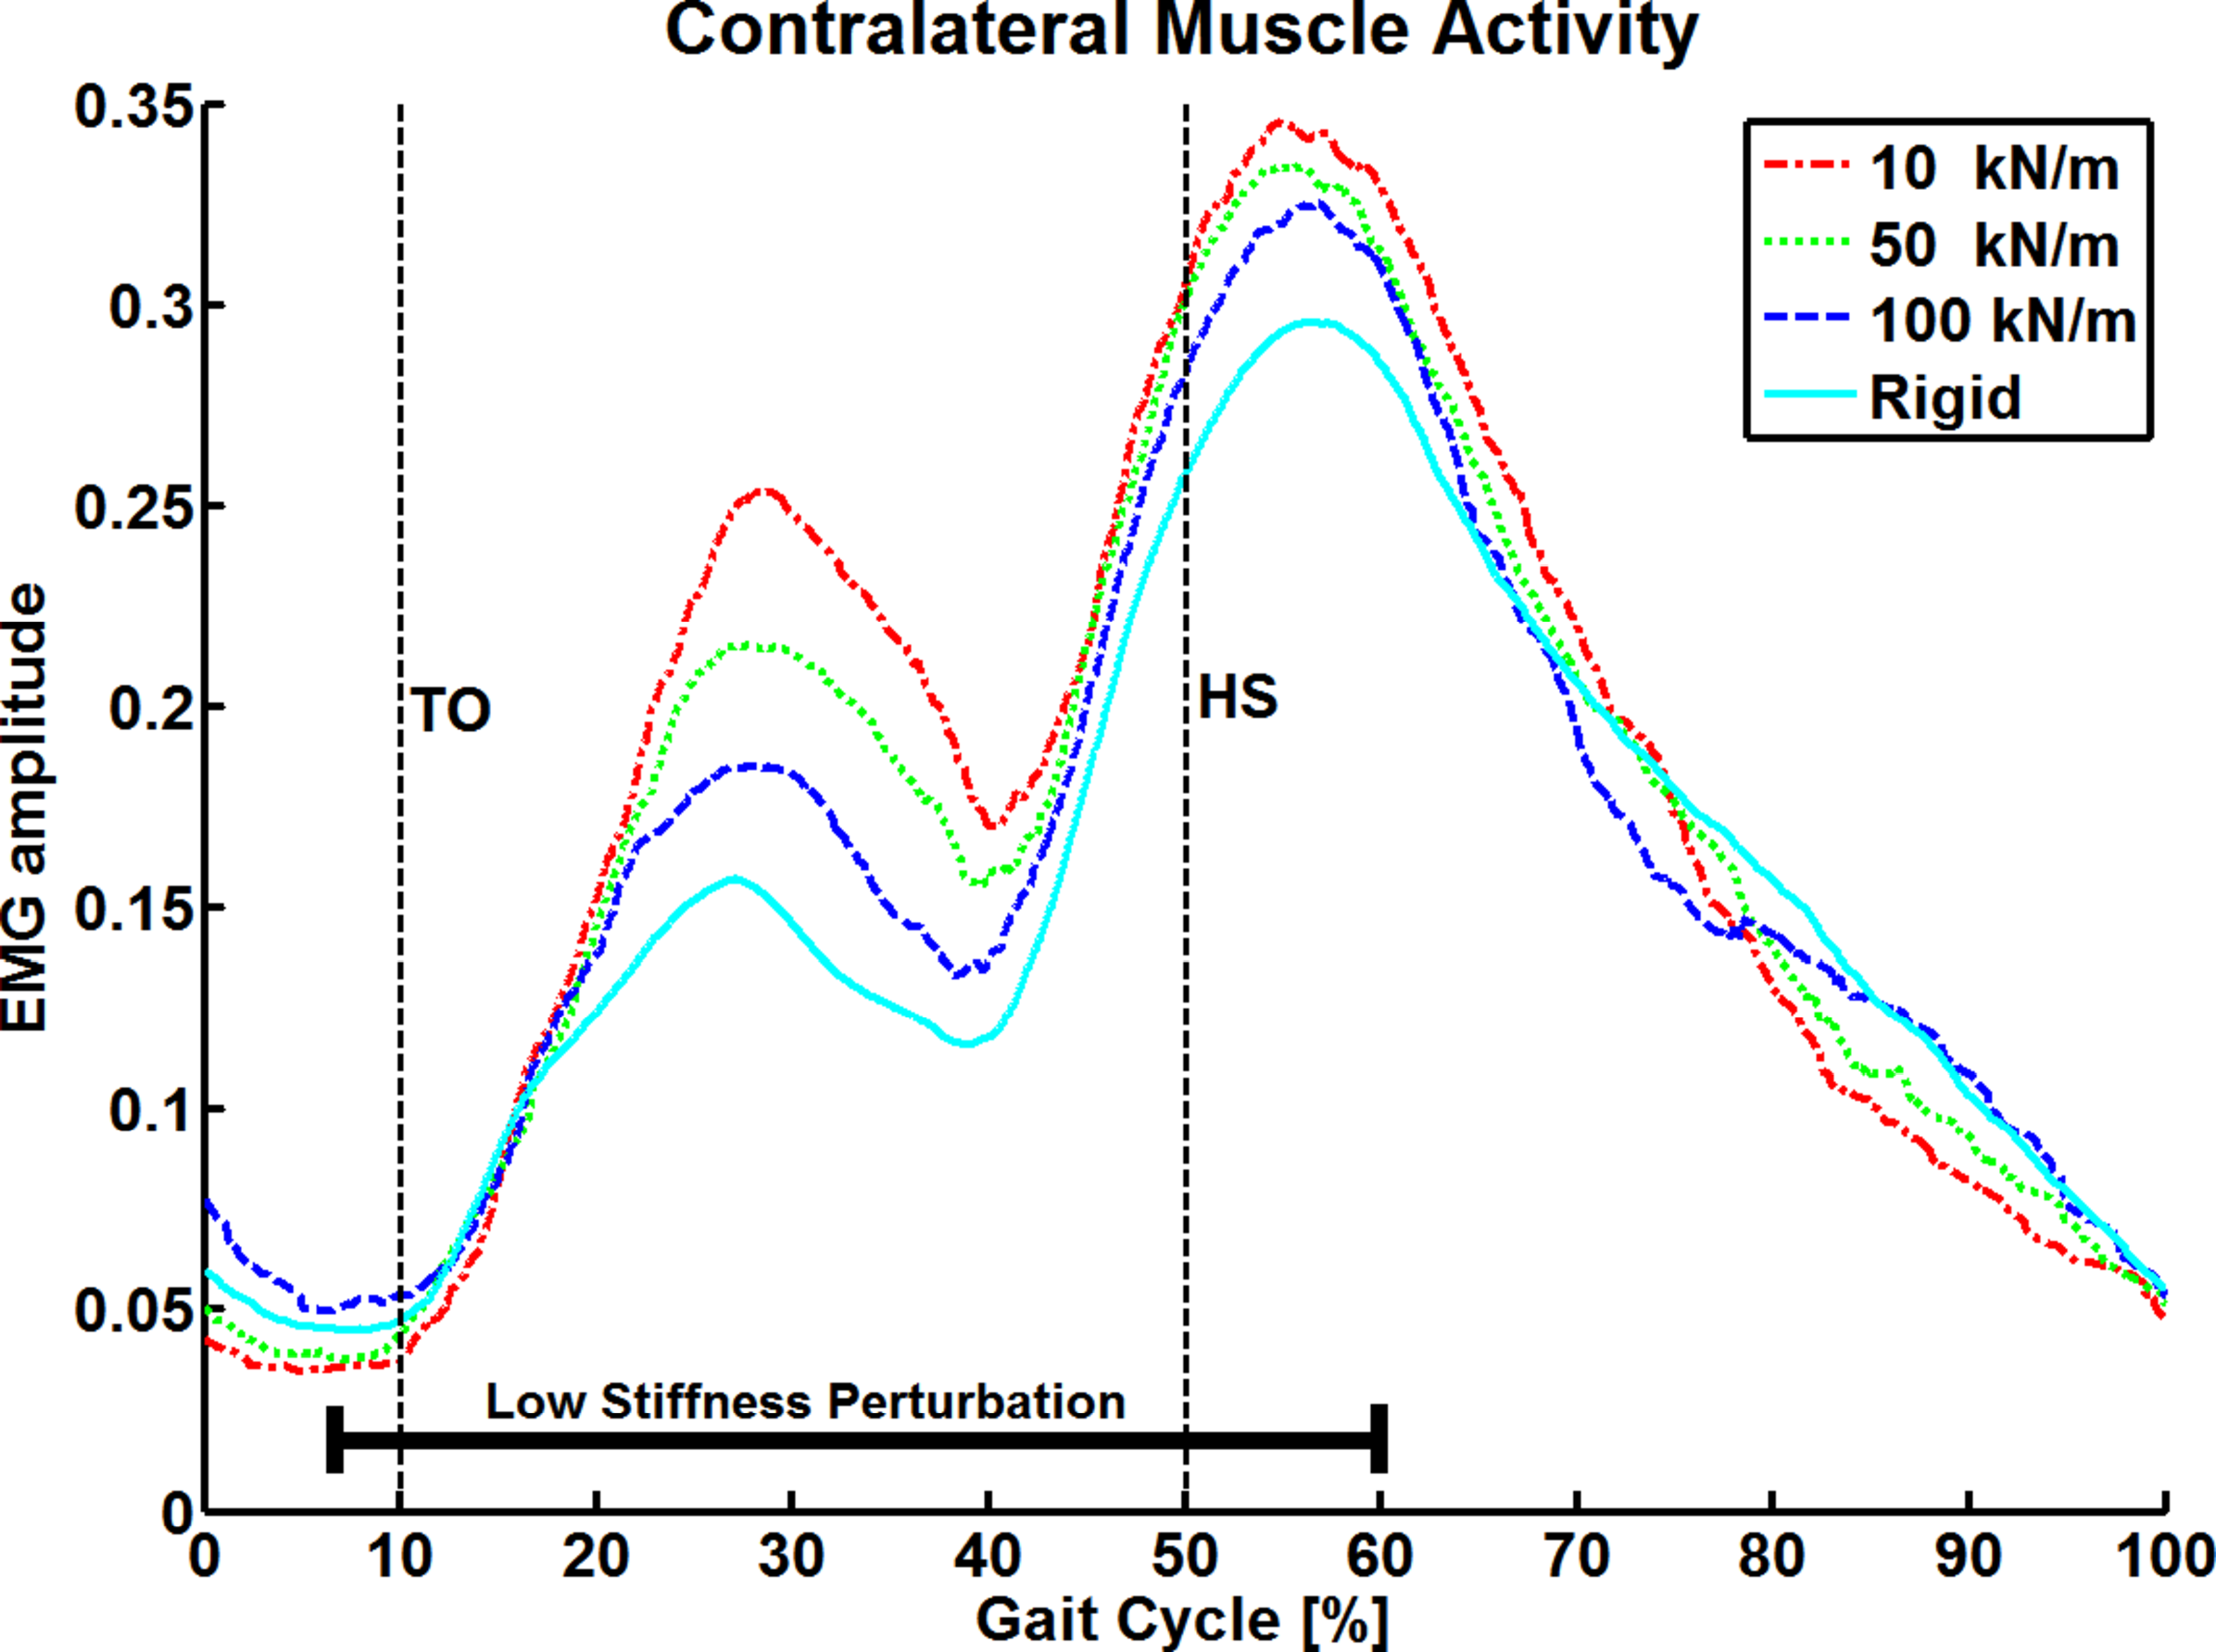
\includegraphics[width=.9\columnwidth]{Figures/TA_all_mean}
	\caption{ \Jc{y units ? } }
	\label{taAllMean}
\end{subfigure}

\vspace{3 mm}

\begin{subfigure}{1.0\columnwidth}
	\centering
	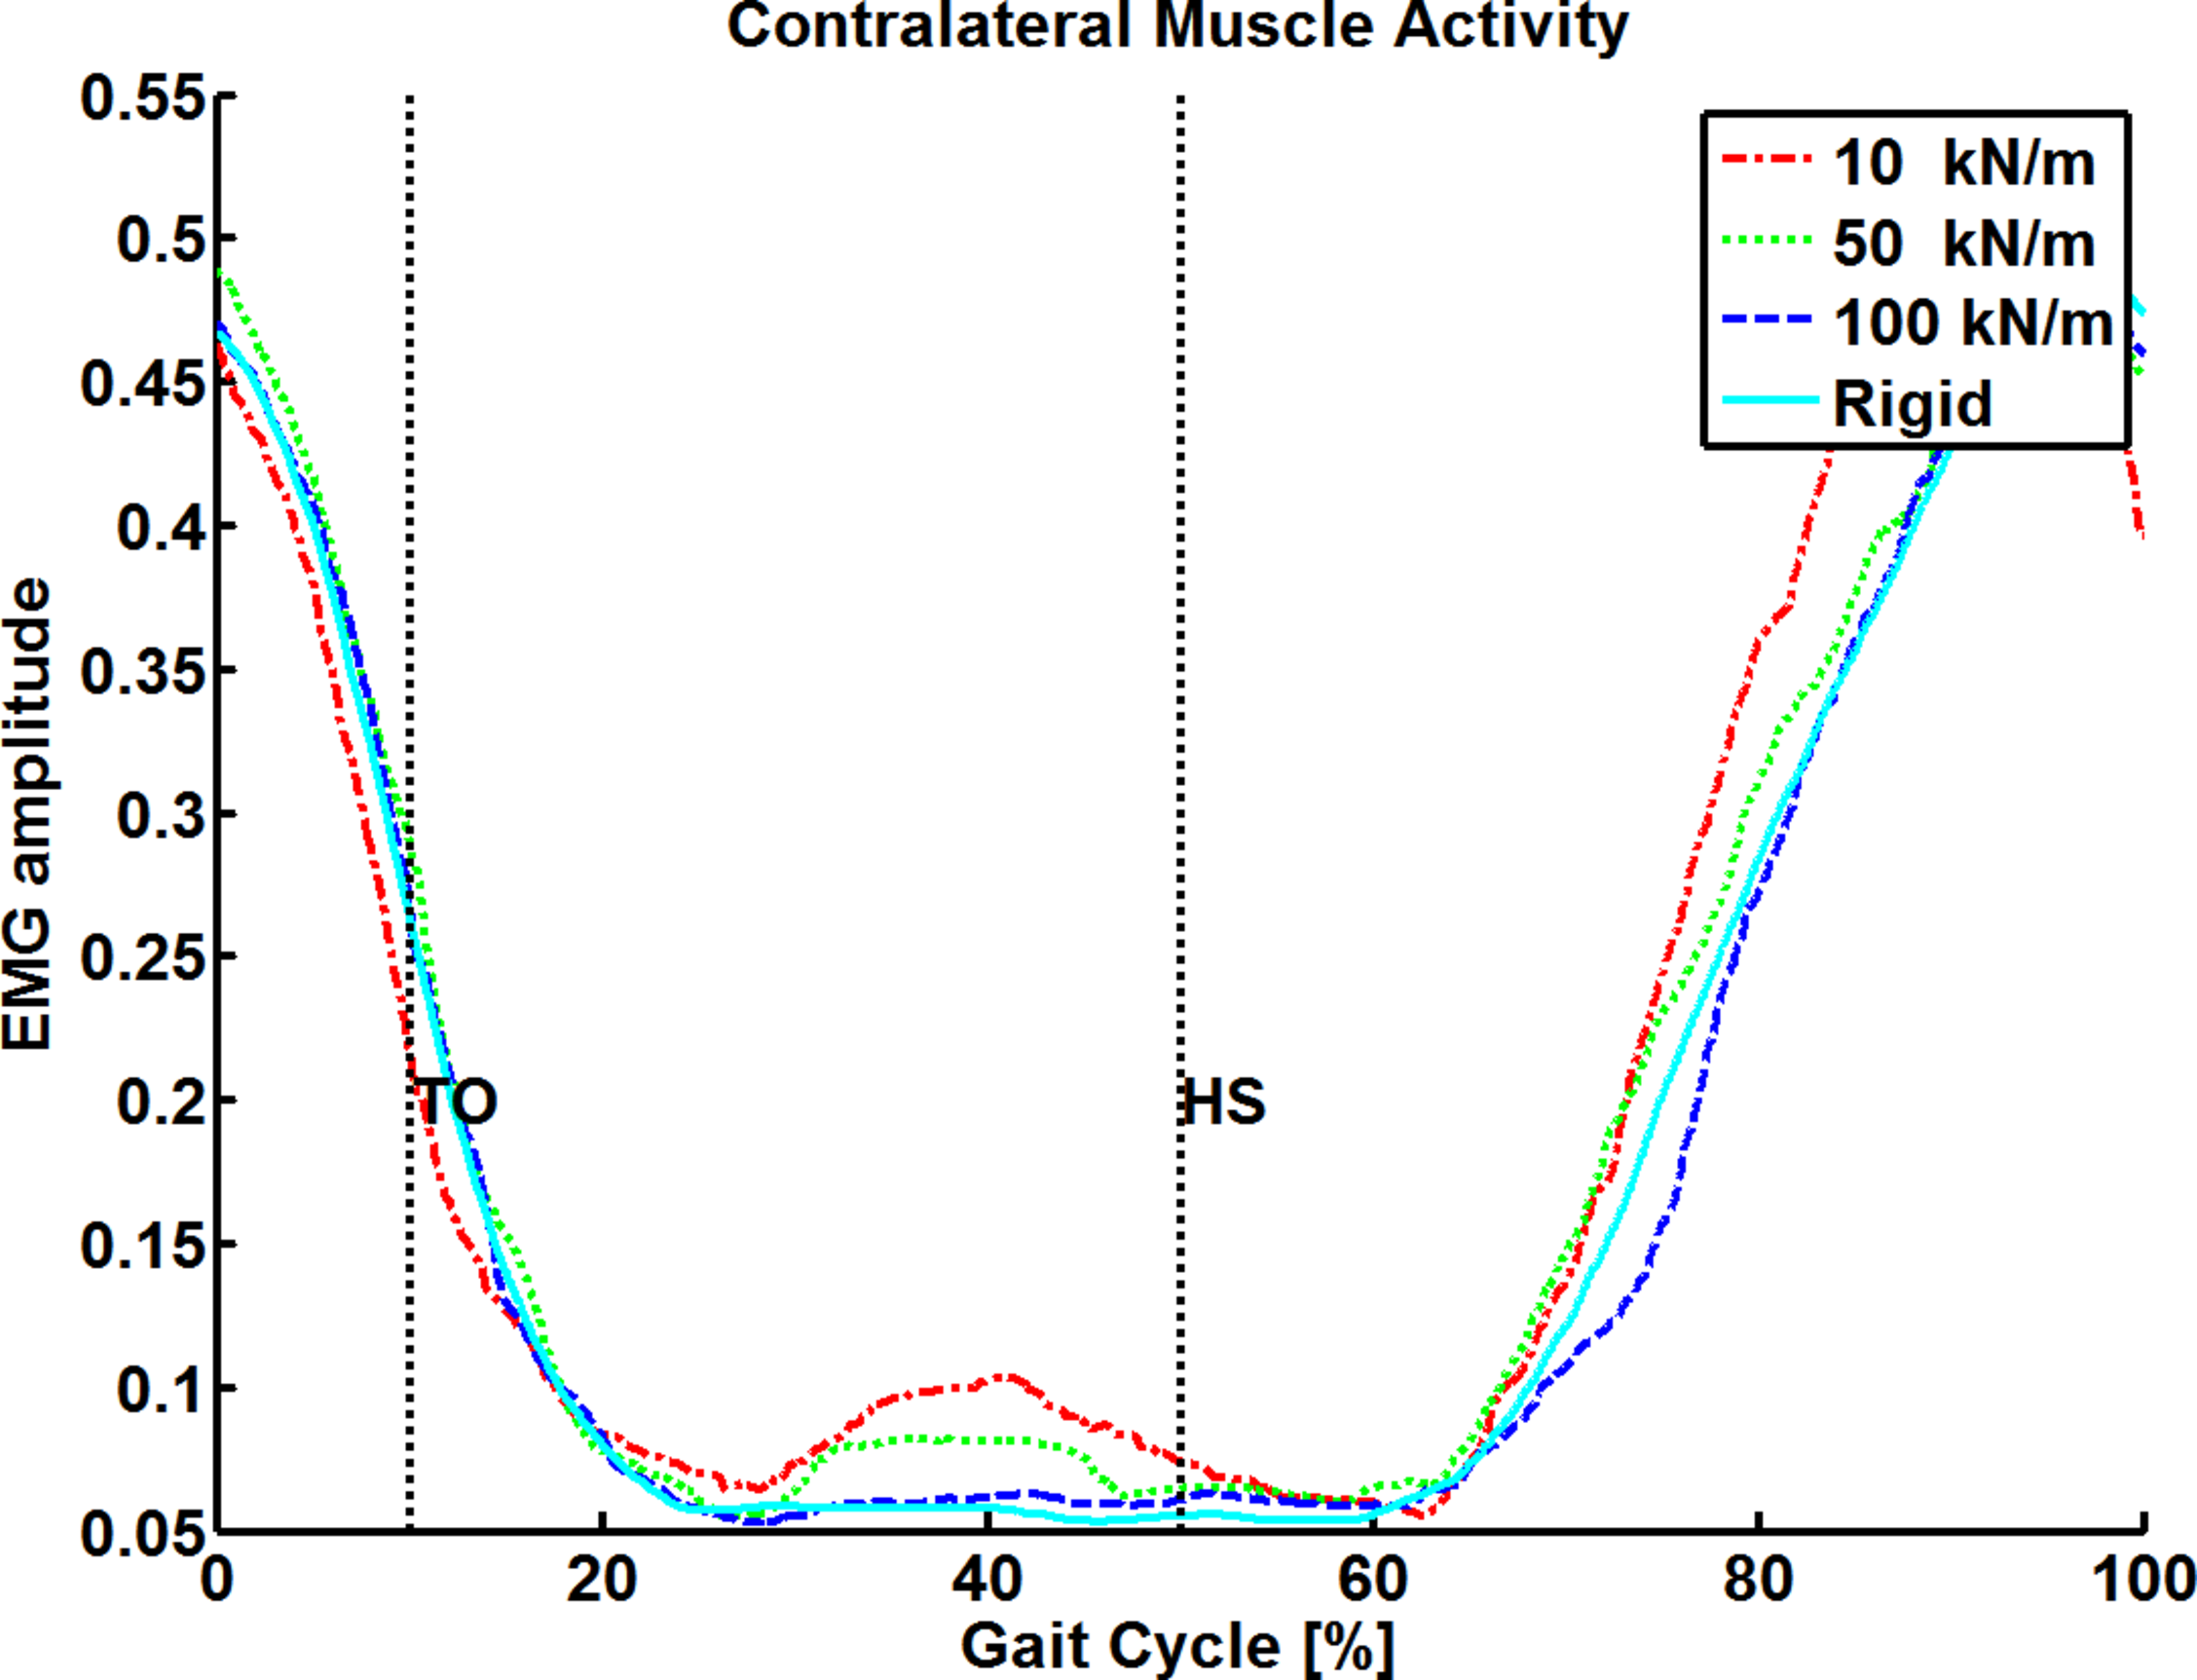
\includegraphics[width=.9\columnwidth]{Figures/GA_all_mean}
	\caption{\Jc{Modify to look like (a), shift data 5}}
	\label{gaAllMean}
\end{subfigure}

\vspace{3 mm}

\begin{subfigure}{1.0\columnwidth}
	\centering
	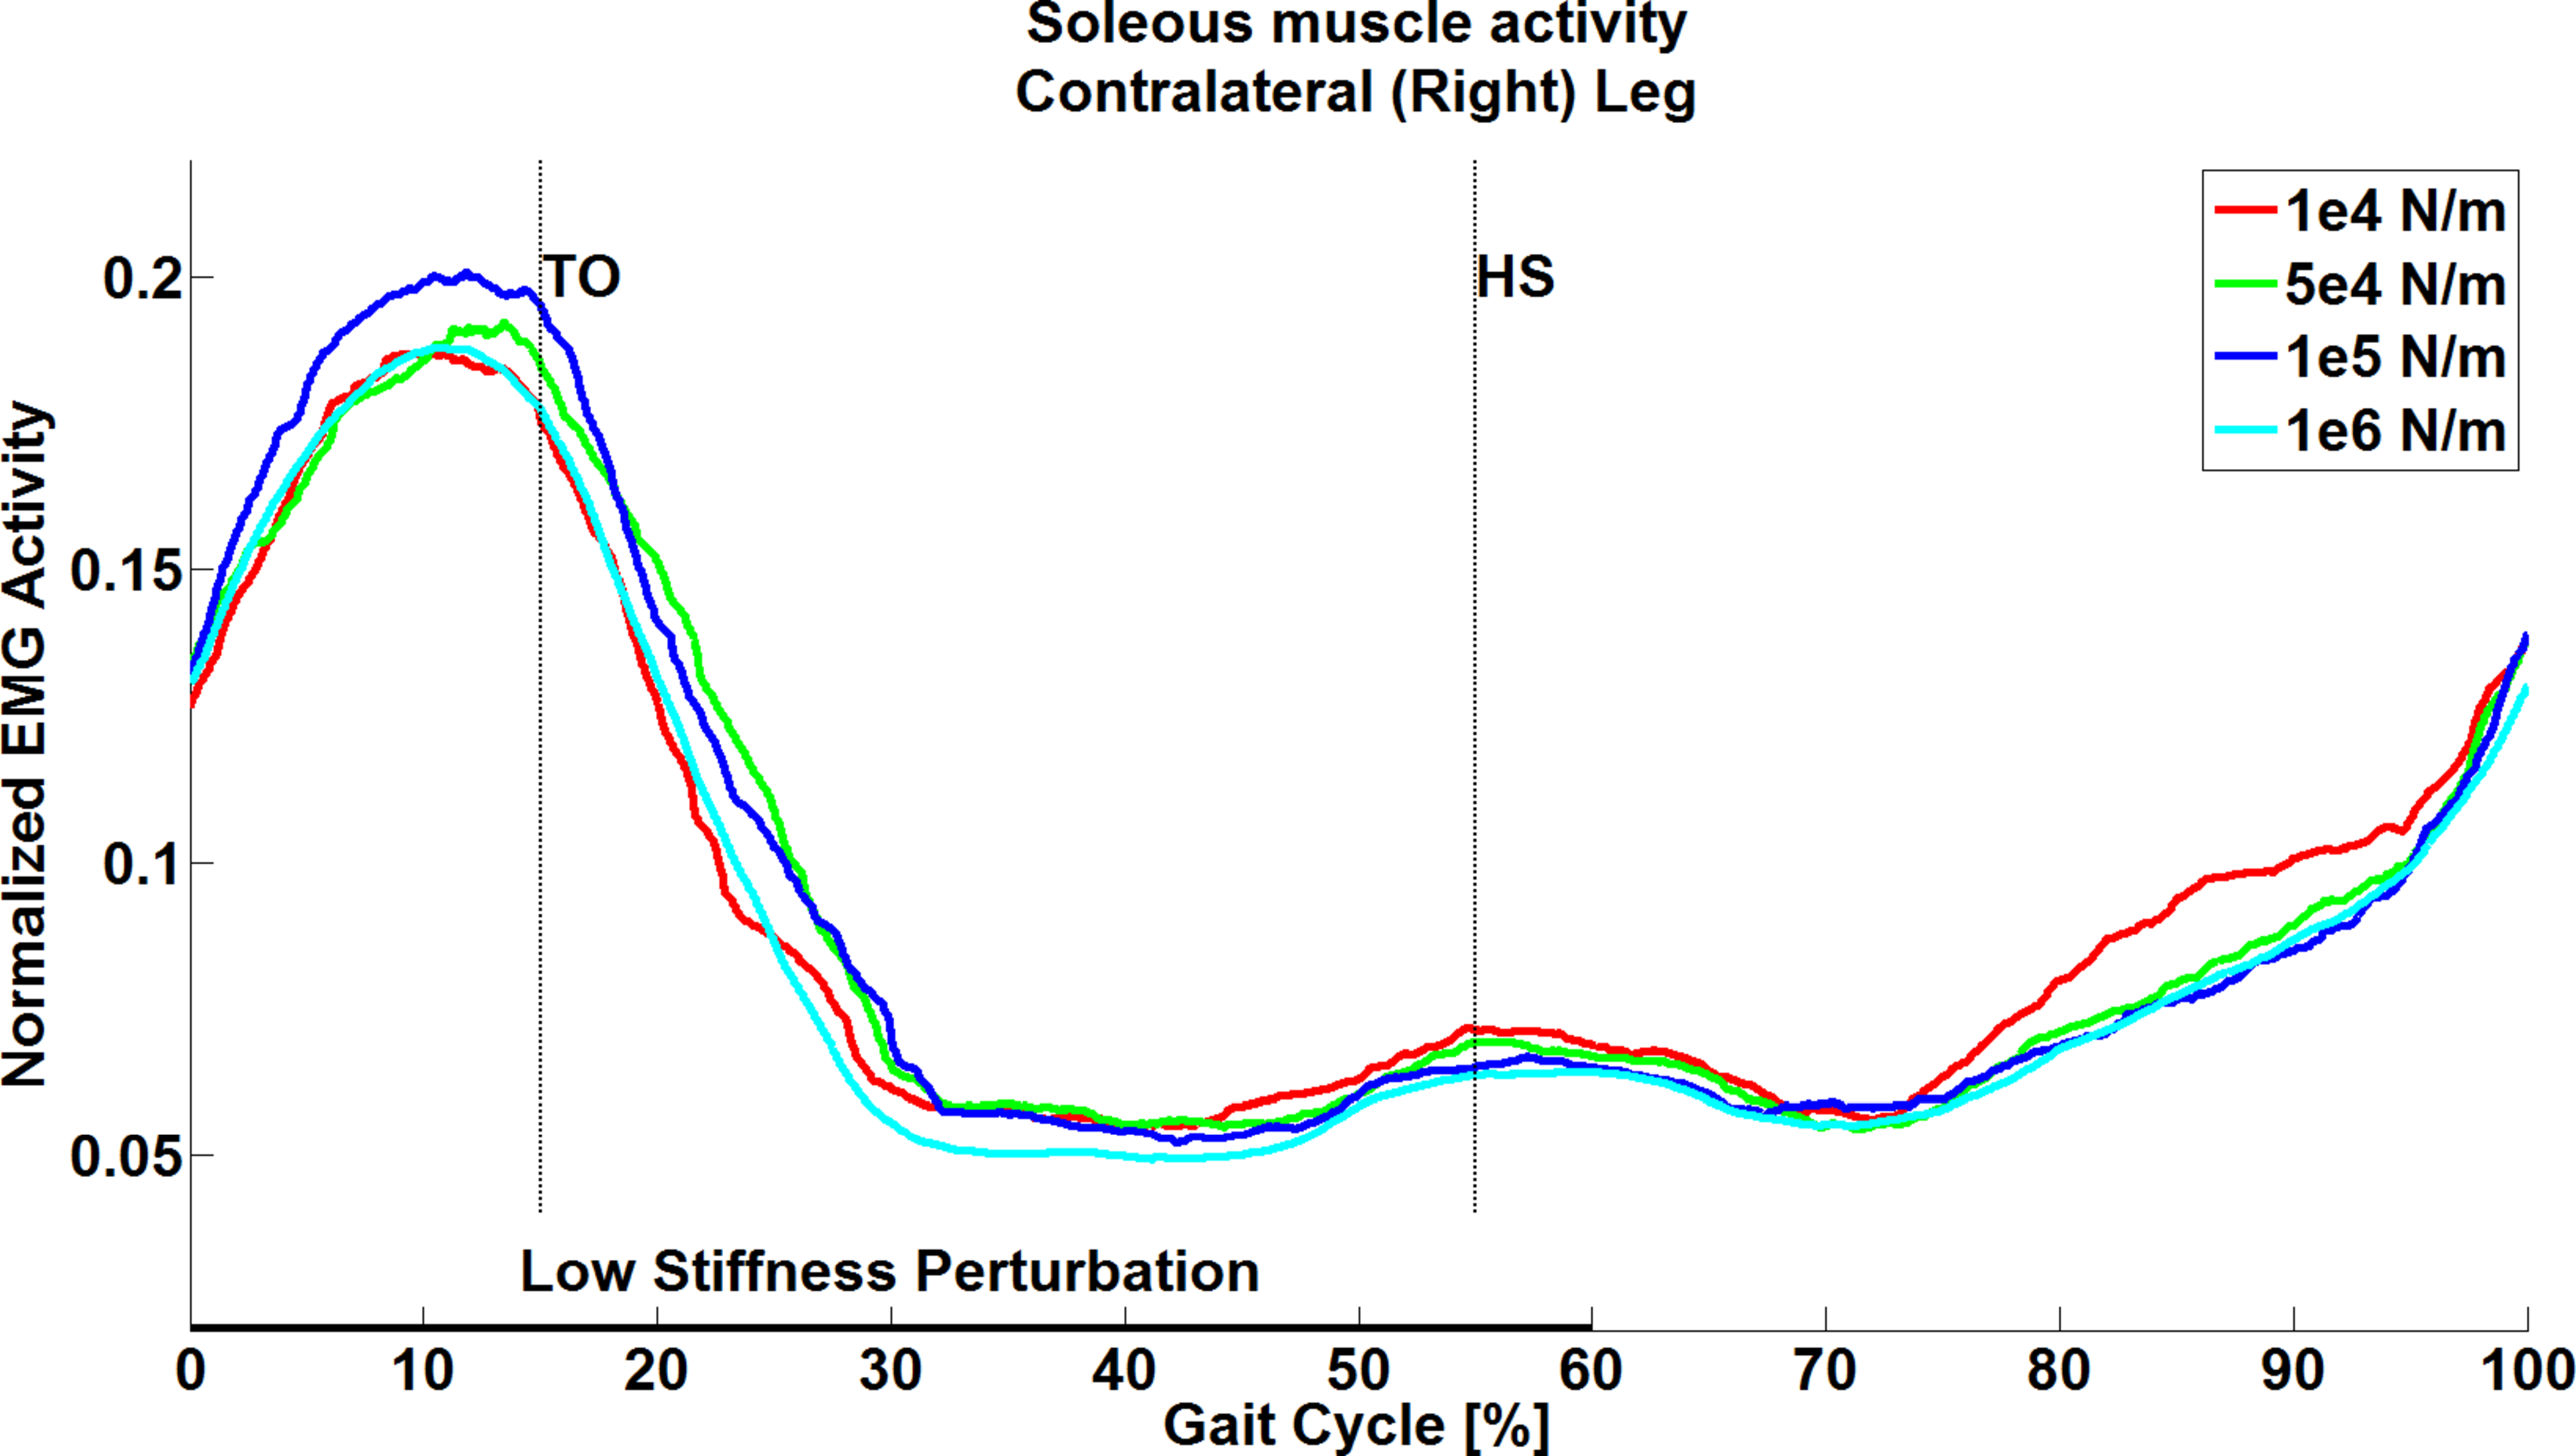
\includegraphics[width=.9\columnwidth]{Figures/SOL_all_mean}
	\caption{\Jc{Modify to look like (a), shift data 5}}
	\label{solAllMean}
\end{subfigure}

\caption{Averaged muscle activity of right leg of a representative subject for the (a) Tibialis Anterior (b) Gastrocnemius and (c) Soleous. Mean values are shown along with an indication of the timing of the perturbation. $100\%$ of the gait cycle corresponds to approx. $1.6\,s$.}
\label{muscleActivityFigure}
\end{figure}
